%% ΕΞΩΤΕΡΙΚΑ ΕΡΓΑΛΕΙΑ
%% Σε αυτό το κεφάλαιο γίνεται περιγραφή των υπόλοιπων εξωτερικών
%% εργαλείων που χρησιμοποιήθηκαν από για την υλοποίηση του συστήματος
%% κρατήσεων ραντεβού.

\chapter{Εξωτερικά Εργαλεία}
Εκτός του Calendar API και των βιβλιοθηκών που παρέχει η Google, έχουν χρησιμοποιηθεί και κάποια άλλα εργαλεία ανάπτυξης λογισμικού τα οποία βοήθησαν στην άρτια και ποιοτικότερη παραγωγή του συστήματος κρατήσεων ραντεβού. Τα εργαλεία αυτά είναι όλα ανοιχτού κώδικα (open source) και έχουν στόχο να βοηθήσουν τον προγραμματιστή να επικεντρωθεί περισσότερο σε αυτό που έχει να κάνει και όχι τόσο στα τετριμμένα πράγματα τα οποία αποσπούν μεγάλο χρονικό διάστημα άσκοπα. Εν ολίγοις πρόκειται για ένα σύνολο από διάφορα framework τα οποία είναι πολύ χρήσιμα για οποιαδήποτε ανάπτυξη λογισμικού.

\section{CodeIgniter}
Το CodeIgniter είναι ένα PHP framework το οποίο έχει ως στόχο την αποδοτικότητα και την ταχύτητα μιας και καταναλώνει πολύ λίγους υπολογιστικούς πόρους σε αντίθεση με άλλα βοηθητικά συστήματα του είδους του. Θετικό στοιχείο είναι ότι είναι πολύ απλό στην χρήση, δίνει την δυνατότητα στον προγραμματιστή να παραμετροποιήσει τον πυρήνα του καταπώς τον βολεύει και βασίζεται στην αρχιτεκτονική MVC (Model - View - Controller). Όντας έργο ανοιχτού λογισμικού κατέχει μια μεγάλη κοινότητα που το υποστηρίζει και επίσης προσφέρει μια καλά ενημερωμένη γνωσιακή βάση, η οποία μπορεί να καθοδηγήσει τον προγραμματιστή στο πως θα χρησιμοποιήσει το framework.

Η αρχιτεκτονική MVC είναι η πλέον διαδεδομένη κυρίως στις διαδικτυακές εφαρμογές αφού αποσκοπεί στην καλύτερη οργάνωση και συντήρηση του κώδικα. Ουσιαστικά πρόκειται για τον διαχωρισμό της εφαρμογής σε τρία μέρη:
\begin{enumerate}
\item Models: Περιέχουν συναρτήσεις και μεθόδους που αλληλεπιδρούν με την βάση δεδομένων. Χρησιμοποιούνται σε διάφορες περιπτώσεις από τους Controllers. Με αυτόν τον τρόπο επιτυγχάνεται η επαναχρησιμοποίηση ενός μέρους του κώδικα, κάτι το οποίο είναι πολύ σημαντικό στην αρχιτεκτονική ενός συστήματος.
\item Views: Τα views είναι τα κομμάτια κώδικα τα οποία παράγουν το αποτέλεσμα το οποίο βλέπει ο χρήστης κάθε φορά. Στόχος τους είναι απλώς να δείξουν και όχι να υπολογίσουν ή να φέρουν κάποια δεδομένα (αυτό είναι δουλειά των άλλων δυο τμημάτων της αρχιτεκτονικής). Κάθε φορά που χρειάζεται να αλλάξει κάτι στην εμφάνιση του συστήματος μπορεί να γίνει αλλαγή στο αντίστοιχο view χωρίς να επηρεαστούν τα άλλα συστήματα. 
\item Controllers: Το μέρος αυτό του συστήματος αναλαμβάνει να οργανώσει τα άλλα δυο. Κάθε φορά που πρέπει να παραχθεί μια σελίδα η διαδικασία θα ξεκινήσει από τον αντίστοιχο controller. Αυτός στην συνέχεια θα καλέσει τις απαραίτητες συναρτήσεις και θα παρέχει τα δεδομένα που απαιτεί το view για να εμφανιστεί σωστά η σελίδα.
\end{enumerate}

\begin{figure}
\centering
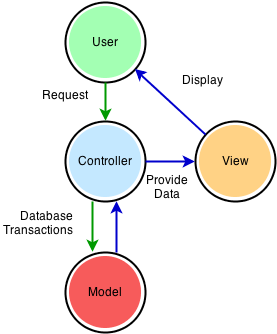
\includegraphics[width=70mm]{images/mvc.png}
\caption{Αρχιτεκτονική MVC}
\label{mvc}
\end{figure}

Το σύστημα που υλοποιήθηκε χρησιμοποιεί το CodeIgniter για την κάλυψη των βασικών εργασιών έτσι ώστε να υπάρχει η δομή MVC στον κώδικα. Επίσης γίνεται χρήση της ενσωματωμένης βιβλιοθήκης επικοινωνίας με την βάση δεδομένων. Εκτός αυτών των δύο, ο υπόλοιπος κώδικας έχει γραφεί κανονικά και τηρεί τις προϋποθέσεις της πτυχιακής εργασίας.

\section {jQuery \& jQuery UI}
Ένα μεγάλο μέρος των σύγχρονων διαδικτυακών εφαρμογών βασίζει την λειτουργία του σε κώδικα JavaScript έτσι ώστε να κάνει το λογισμικό πιο φιλικό προς τον χρήστη. Διάφορες βιβλιοθήκες έχουν δημιουργηθεί τα τελευταία χρόνια που στόχο έχουν την εξέλιξη και την αποδοτικότερη χρήση της γλώσσας JavaScript. Η πιο δημοφιλής από όλες αυτές τις βιβλιοθήκες είναι η jQuery η οποία συνοδεύεται από το jQuery UI, ένα framework για την παραγωγή ελεκτηρίων (controls) στα οποία μπορεί ο κάθε χρήστης να εκτελέσει διάφορες ενέργειες. Το jQuery έχει καταφέρει να απλοποιήσει την συγγραφή JavaScript κώδικα και επιπλέον παρέχει στην διάθεση του προγραμματιστή έτοιμες ρουτίνες animation και διαφόρων άλλων ενεργειών, οι οποίες διαφορετικά θα καταλάμβαναν αρκετό χρόνο για την υλοποίηση τους. Πρόκειται για μια βιβλιοθήκη ανοιχτού λογισμικού η οποία υποστηρίζεται από μια πολύ μεγάλη κοινότητα προγραμματιστών. Υπάρχει επίσης πληθώρα πρόσθετων (plugins) με λειτουργίες οι οποίες δεν είναι διαθέσιμες στην βασική βιβλιοθήκη.

Η jQuery ουσιαστικά λειτουργεί σαν ένα επίπεδο πάνω από την JavaScript βοηθώντας τον προγραμματιστή να γράψει διάφορες δομές κώδικα πιο γρήγορα και οργανωμένα. Ο κώδικας που γράφεται είναι πάλι JavaScript οπότε είναι πολύ εύκολο στον καθένα να χρησιμοποιήσει την βιβλιοθήκη. Στόχος της είναι η πιο εύκολη περιήγηση στα αντικείμενα μιας σελίδας (DOM elements), η εύκολη δημιουργία εφέ κινήσεων τα οποία προσδίδουν πολύ αισθητικά σε μια ιστοσελίδα, η ευκολότερη χρήση της τεχνολογίας AJAX, μιας τεχνολογίας η οποία χρησιμοποιείται όλο και περισσότερο από τα σύγχρονα συστήματα.

Το σύστημα που παράχθηκε χρησιμοποιεί αυτήν την βιβλιοθήκη για τον προγραμματισμό του client-side μέρους της εφαρμογής. Ανάλογα με την κάθε περίσταση, μερικές φορές είναι αποδοτικότερο και χρησιμότερο να χρησιμοποιηθεί JavaScript έναντι της PHP και για αυτόν τον λόγο επιλέγχθηκε το jQuery Framework ως εργαλείο κατά την υλοποίηση του συστήματος.

\section {Bootstrap}
Το Bootstrap είναι ένα ολοκληρωμένο CSS Framework με την προσθήκη κάποιων βιβλιοθηκών JavaScript έτσι ώστε να προσφέρει μερικές επιπλέον δυνατότητες. Έχει κατασκευαστεί από την εταιρεία πίσω από την σελίδα κοινωνικής δικτύωσης Twitter και χρησιμοποιείται από αυτό ως βάση για την υλοποίηση του. Η εταιρεία έχει διαθέσει το framework ως ανοιχτό λογισμικό και οι προγραμματιστές μπορούν να το χρησιμοποιήσουν ελεύθερα στις σελίδες τους. Η ίδια η εταιρεία επωφελείται μέσω της συμμετοχής της κοινότητας για να αναπτύξει περαιτέρω το framework.

Το Bootstrap περιέχει έτοιμο κώδικα CSS ο οποίος ακολουθεί την μεθοδολογία παραγωγής responsive ιστοσελίδων. Με την έννοια αυτή εννοείται ότι η μορφοποίηση των σελίδων στοχεύει στο να είναι συμβατή με οποιαδήποτε συσκευή, λειτουργικό σύστημα και περιηγητή ιστού. Είναι πολύ σημαντικό για την αναγνωρισιμότητα και ευχρηστία μιας εφαρμογής το να είναι διαθέσιμη σε οποιοδήποτε μηχάνημα υποστηρίζει τα τελευταία standards του ιστού. Το JavaScript μέρος του framework χρησιμοποιεί το jQuery για την υλοποίηση διαφόρων τεχνικών (πχ εμφάνιση παραθύρου διαλόγου).

Στην παραγωγή του συστήματος κρατήσεων ραντεβού χρησιμοποιήθηκε ως η βάση για τη μορφοποίηση και κάποιες μέθοδοι JavaScript φάνηκαν αρκετά χρήσιμα σε κάποια σημεία. Στην συνέχεια με βάση αυτά γράφτηκαν ξεχωριστά αρχεία CSS και JavaScript τα οποία αποτελούν το τελικό αποτέλεσμα που έπρεπε να επιτευχθεί. 